\documentclass{standalone}
%\usepackage{amsmath}\usepackage{lmodern}      % Matches the MathJax default (Latin Modern)
%\usepackage[T1]{fontenc}  % Ensures proper character encoding
\usepackage{tikz}
\usetikzlibrary{positioning, arrows.meta, calc}

% Document metadata (Safe to keep in preamble, standalone will skip them during crop)
\title{Chapter 07 — section 12 — diagram 04}
\author{0im}
\date{2026}

\begin{document}
    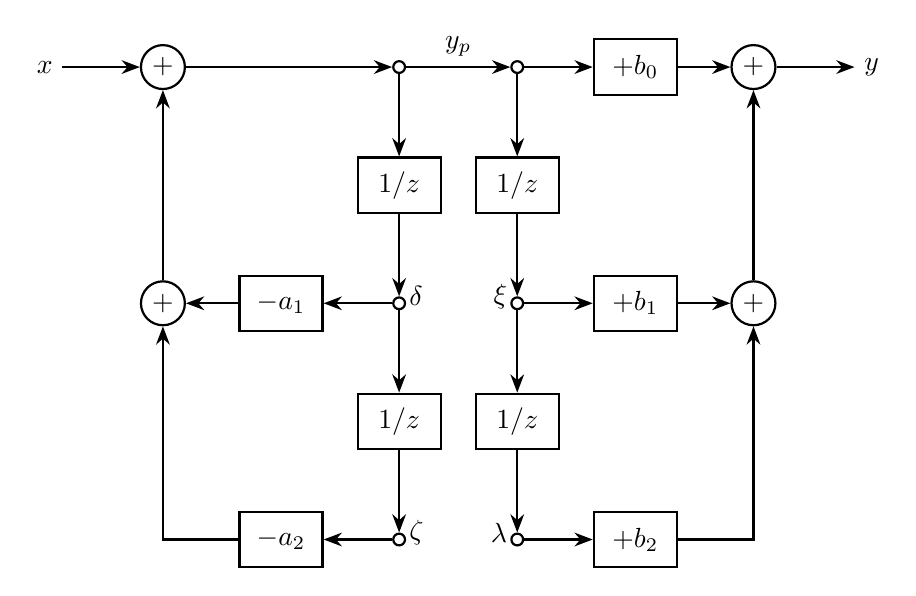
\begin{tikzpicture}
    [
        on grid, 
        node distance=1.5cm and 1.5cm, % Fixed: Added explicit cm units
        block/.style={draw, rectangle, minimum height=2em, minimum width=3em, thick},
        sum/.style={draw, circle, inner sep=2pt, thick},
        branch/.style={draw, circle, inner sep=1.5pt, thick}
    ]
        % =========================================================================
        % NODES
        % =========================================================================
        % --- Row 1 ---
        \node (x) {$x$};
        \node [sum, right=of x] (sum1) {$+$};
        \node [right=of sum1] (blank1_3) {};
        \node [branch, right=of blank1_3] (branch1) {};
        \node [branch, right=of branch1] (branch2) {};
        \node [block, right=of branch2] (b0) {$+b_0$};
        \node [sum, right=of b0] (sum2) {$+$};
        \node [right=of sum2] (y) {$y$};        
        % --- Row 2 ---
        \node [below=of sum1] (blank2_2) {};
        \node [below=of blank1_3] (blank2_3) {};
        \node [block, below=of branch1] (z1L) {$1/z$};
        \node [block, below=of branch2] (z1R) {$1/z$};
        \node [below=of b0] (blank2_6) {};
        \node [below=of sum2] (blank2_7) {};        
        % --- Row 3 ---
        \node [sum, below=of blank2_2] (sum3) {$+$};
        \node [block, below=of blank2_3] (a1) {$-a_1$};
        \node [branch, below=of z1L] (branch3) {};
        \node [branch, below=of z1R] (branch4) {};
        \node [block, below=of blank2_6] (b1) {$+b_1$};
        \node [sum, below=of blank2_7] (sum4) {$+$};        
        % --- Row 4 ---
        \node [below=of sum3] (blank4_2) {};
        \node [below=of a1] (blank4_3) {};
        \node [block, below=of branch3] (z2L) {$1/z$};
        \node [block, below=of branch4] (z2R) {$1/z$};
        \node [below=of b1] (blank4_6) {};
        \node [below=of sum4] (blank4_7) {};        
        % --- Row 5 ---
        \node [below=of blank4_2] (blank5_2) {};
        \node [block, below=of blank4_3] (a2) {$-a_2$};
        \node [branch, below=of z2L] (branch5) {};
        \node [branch, below=of z2R] (branch6) {};
        \node [block, below=of blank4_6] (b2) {$+b_2$};
        \node [below=of blank4_7] (blank5_7) {};
        
        % =========================================================================
        % PATHS
        % =========================================================================
        % --- HORIZONTAL ---
        %  Row 1
        \draw [-Stealth, thick] (x) -- (sum1);
        \draw [-Stealth, thick] (sum1.east) -- (branch1.west);
        \draw [-Stealth, thick] (branch1.east) -- node [above] {$y_p$} (branch2.west);
        \draw [-Stealth, thick] (branch2.east) -- (b0.west);
        \draw [-Stealth, thick] (b0.east) -- (sum2.west);
        \draw [-Stealth, thick] (sum2.east) -- (y.west);
        %  Row 3
        \draw [-Stealth, thick] (a1.west) -- (sum3.east);
        \draw [-Stealth, thick] (branch3.west) -- (a1.east);
        \draw [-Stealth, thick] (branch4.east) -- (b1.west);
        \draw [-Stealth, thick] (b1.east) -- (sum4.west);
        %  Row 5
        \draw [-Stealth, thick] (branch5.west) -- (a2.east);
        \draw [-Stealth, thick] (branch6.east) -- (b2.west);
        % --- VERTICAL ---
        %  Column 1
        \draw [-Stealth, thick] (sum3.north) -- (sum1.south);
        %  Column 2
        \draw [-Stealth, thick] (branch1.south) -- (z1L.north);
        \draw [-Stealth, thick] (z1L.south) -- (branch3.north) node [anchor=west] {$\delta$};
        \draw [-Stealth, thick] (branch3.south) -- (z2L.north);
        \draw [-Stealth, thick] (z2L.south) -- (branch5.north) node [anchor=west] {$\zeta$};
        %  Column 3
        \draw [-Stealth, thick] (branch2.south) -- (z1R.north);
        \draw [-Stealth, thick] (z1R.south) -- (branch4.north) node [anchor=east] {$\xi$};
        \draw [-Stealth, thick] (branch4.south) -- (z2R.north);
        \draw [-Stealth, thick] (z2R.south) -- (branch6.north) node [anchor=east] {$\lambda$};
        %  Column 4
        \draw [-Stealth, thick] (sum4.north) -- (sum2.south);
        % --- ANGLED ---
        \draw [-Stealth, thick] (a2.west) -- (blank5_2.center) -- (sum3.south);
        \draw [-Stealth, thick] (b2.east) -- (blank5_7.center) -- (sum4.south);

    \end{tikzpicture}

\end{document}